\chapter{Single fiber simulations}

Although coarse-grained models of a similar nature can and have been fitted to match the properties of a CNT \cite{Cranford2010}, here we focus on exploring the behavior of the model. To that end we are interested in four stages of the model. First, under what circumstances will a fiber not crystallize with the bottom substrate. Second, what configurations or modes of failure are relevant and observable from various loads applied to the fiber by the top substrate. Third, after being equilibrated in an adhered state (that is, the top substrate adhered to the fiber), what kinds of loads are required to detach the top substrate from the fiber and what configurations are observable intermittently. Finally, if the fiber does successfully detach, under what circumstances will it not crystallize with the bottom substrate.

\section{Free standing}

	\begin{figure}
		\begin{center}
			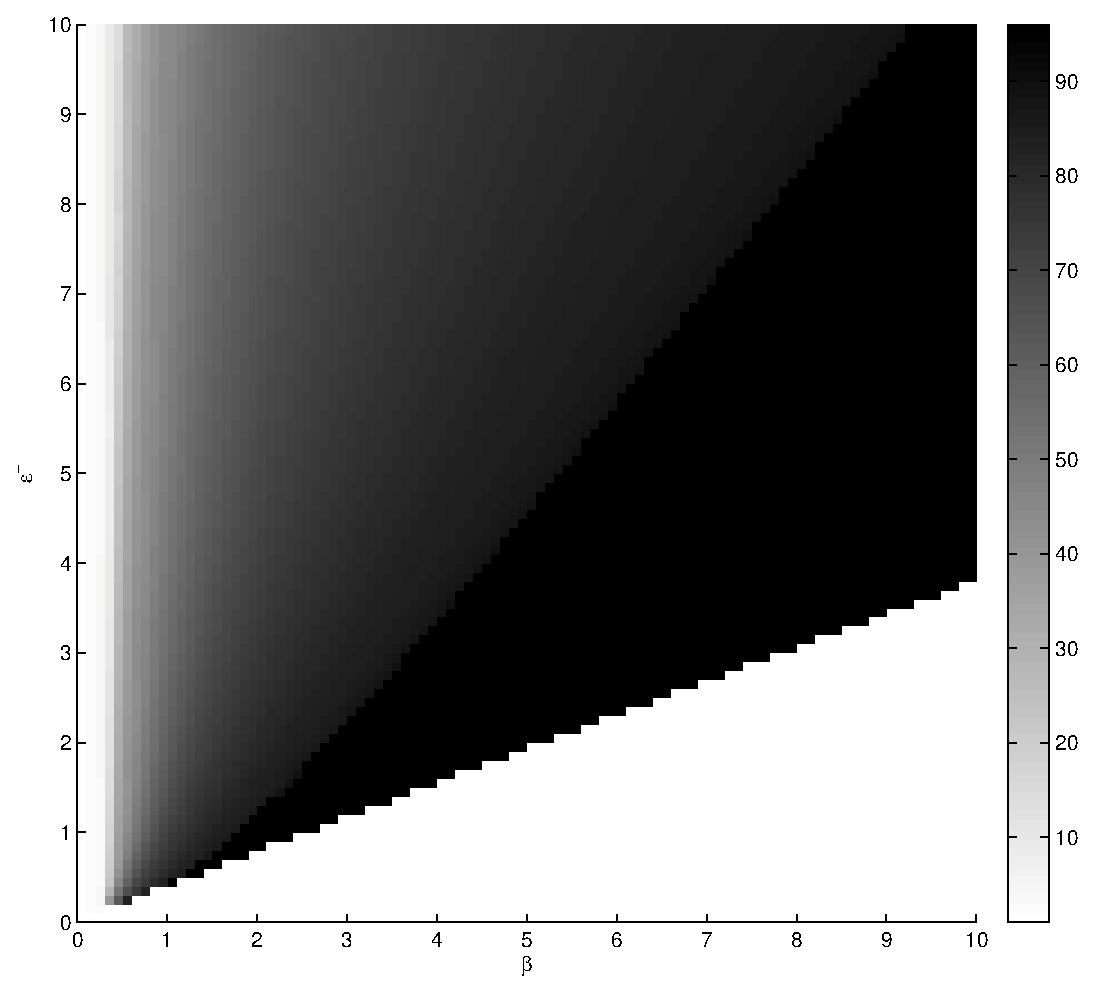
\includegraphics[scale=.5]{./fig/sims/freestanding/fs.eps}
		\end{center}		
		\caption{Phase plot of a fiber's torsional spring strength, $\beta$, against the strength of the bottom substrate's vdW force, $\eps^-$.
		\label{fig:FreeStandingGrid}}
	\end{figure}	

We say a fiber, or part of a fiber, is \textit{crystallized} if the van der Waals energy between a set of particles appears qualitatively to be minimized. If a particle on the fiber is crystallized with two particles on the top substrate we say that it is \textit{adhered} to the top substrate. We define a function to describe how adhered a fiber is to the top substrate in general. Therefore, we define


\begin{eqnarray}
	A(\textbf{a}, \textbf{b}) = \left\{ 
		\begin{array}{ll}
			1, & \|\textbf{a} - \textbf{b}\| \leq 2^{\frac{1}{6}} \sigma + 10^{-6}\\
			0, & \mbox{otherwise}
		\end{array}
		\right.  \\
	A^+ = \sum_{k=1}^{n^+} \sum_{j=1}^{m} \sum_{i=1}^{n} A(\textbf{r}_i^{(j)},\textbf{r}_k^{(+)}) \label{eqn:adhesion:top} \\ 
	A^- = \sum_{k=1}^{n^-} \sum_{j=1}^{m} \sum_{i=1}^{n} A(\textbf{r}_i^{(j)},\textbf{r}_k^{(-)}) \label{eqn:adhesion:bottom}
\end{eqnarray}

If a fiber is not strong enough to prevent crystallization with the bottom substrate without external influence then it is impossible that the fiber will be about to recover from a detachment force. Moreover, the compression with the top substrate will be uninteresting if the fiber is already laying flat in a position the substrate can not effect. Therefore it is pertinent to categorize what parameters cause a fiber to stay upright or at least not crystallize in some capacity. Here we show that $\beta$ and $\eps^-$ play the key role in whether or not the fiber crystallizes (Fig.~\ref{fig:FreeStandingGrid}). The only other parameters that could play a role are: $\sigma$, $\ell$, $\eps$, and $gamma$. With the exception of $\eps$ none of these parameters will have any effect on keeping the fiber standing, but more how the fiber crystallizes or stacks with the bottom substrate. The inner fiber van der Waals interaction strength, $\eps$, is assumed to play a negligible role.

The modes a fiber free from the top substrate are categorizable as collapsed, folded, crystallized, and slanted. These can be immediately seen in figure \ref{fig:FreeStandingGrid}. The white section sufficiently distant from the origin is slanted, the black section above it collapsed, and sufficiently close to the y-axis is crystallized.

	%% Erect Figures
	\begin{figure*}
		\centering
		\begin{subfigure}{.5\textwidth}
			\centering
			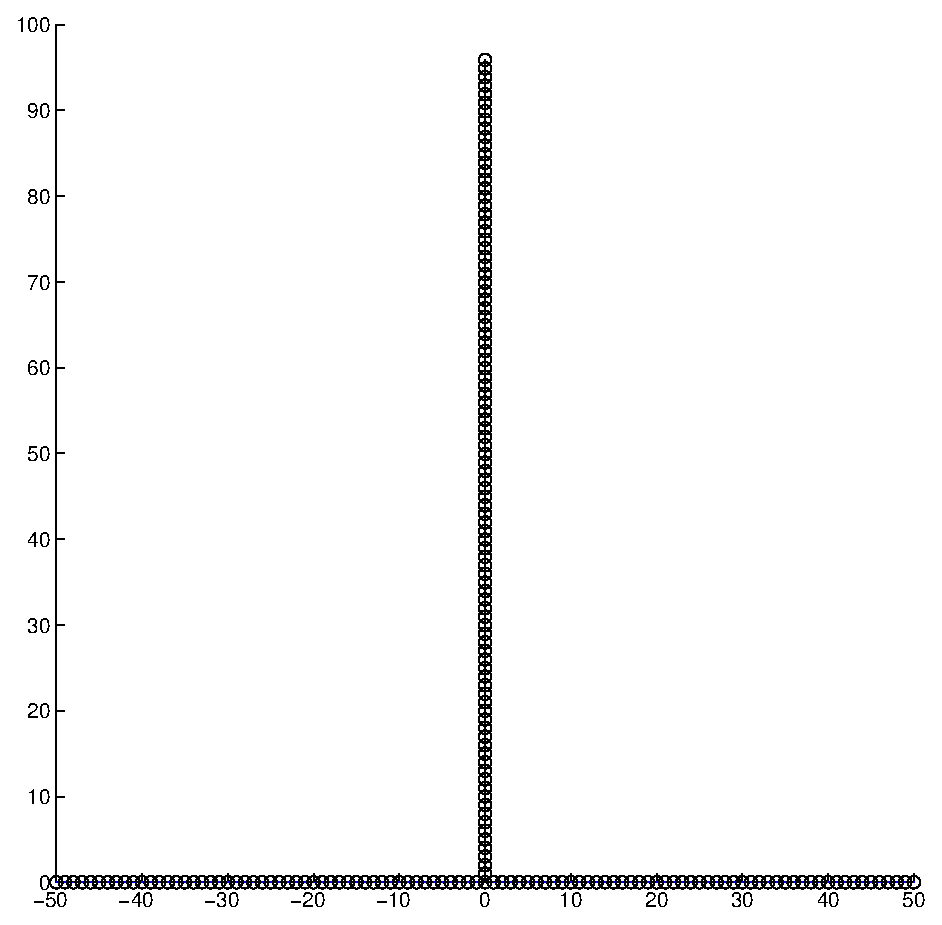
\includegraphics[scale=.4]{./fig/sims/freestanding/erect.eps}
			\caption{TODO \label{subfig:fs_erect}}
		\end{subfigure}%
		~
		\begin{subfigure}{.5\textwidth}
			\centering
			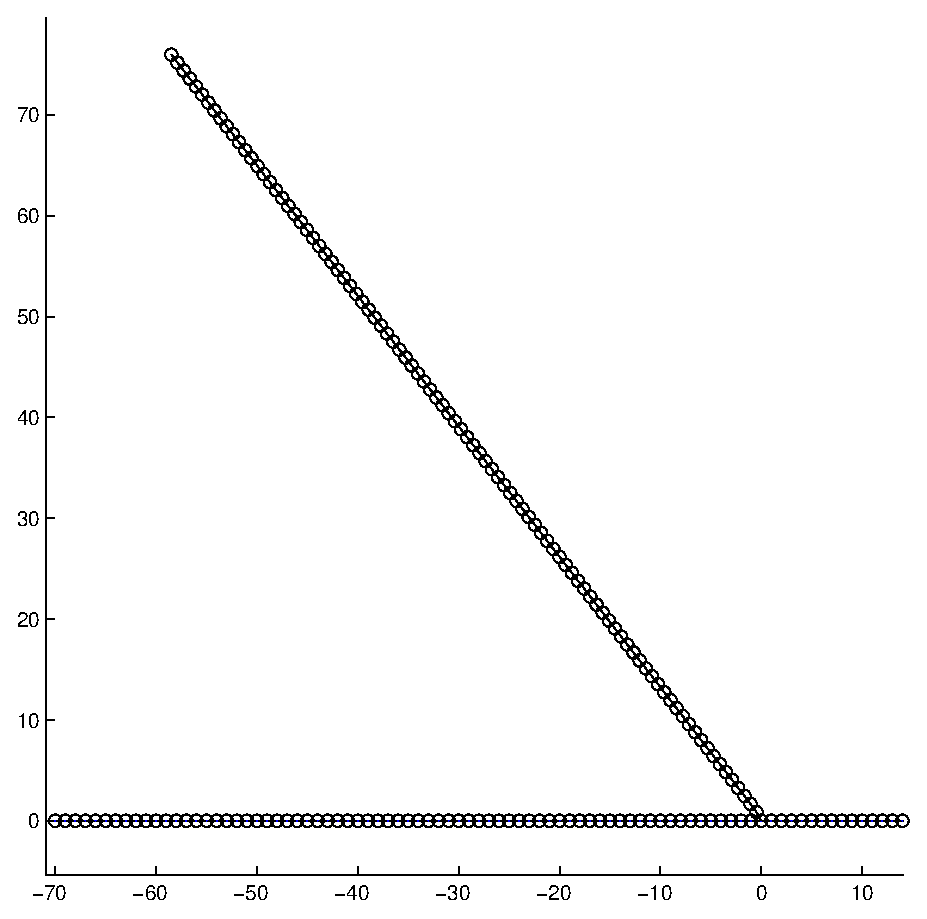
\includegraphics[scale=.4]{./fig/sims/freestanding/erect_leaning.eps}
			\caption{TODO\label{subfig:fs_erectlean}}
		\end{subfigure}
		\caption{TODO\label{fig:fs_erect}}
	\end{figure*}
	
	%% Fallen Figures
	\begin{figure*}
		\centering
		\begin{subfigure}{.5\textwidth}
			\centering
			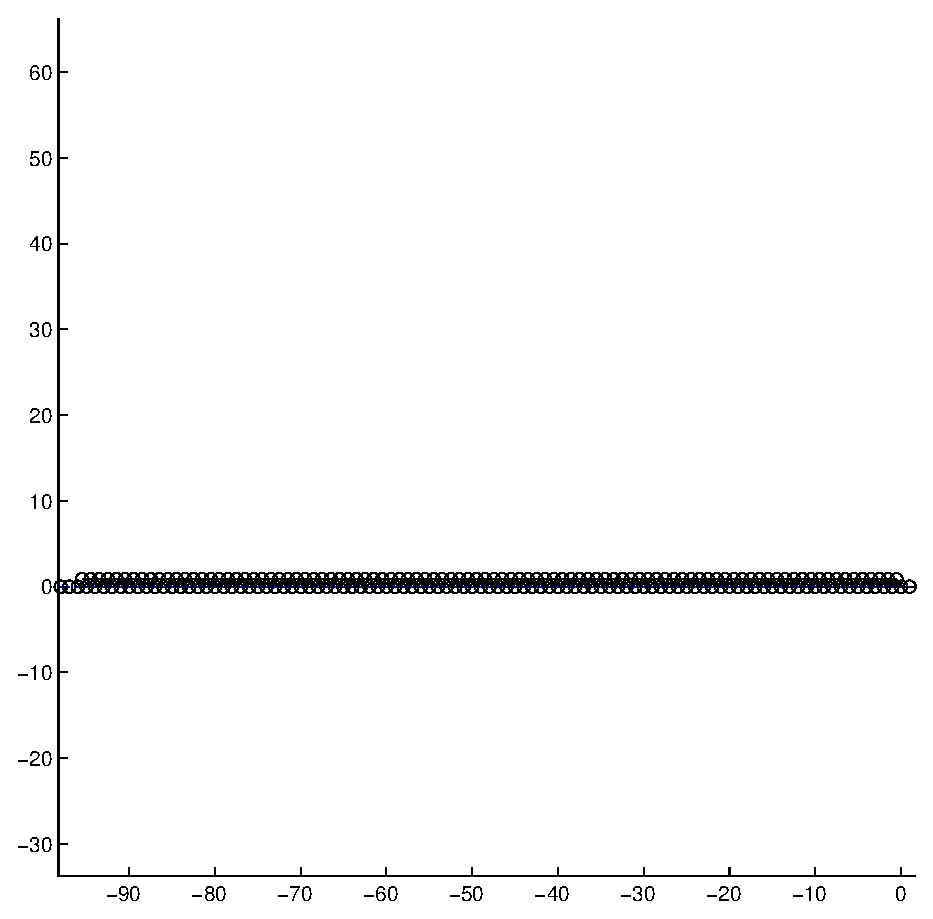
\includegraphics[scale=.4]{./fig/sims/freestanding/completely_down.eps}
			\caption{TODO \label{subfig:fs_down}}
		\end{subfigure}%
		~
		\begin{subfigure}{.5\textwidth}
			\centering
			\includegraphics[scale=.4]{./fig/sims/freestanding/one_fold.eps}
			\caption{TODO \label{subfig:fs_onefold}}
		\end{subfigure}

		\begin{subfigure}{.5\textwidth}
			\centering
			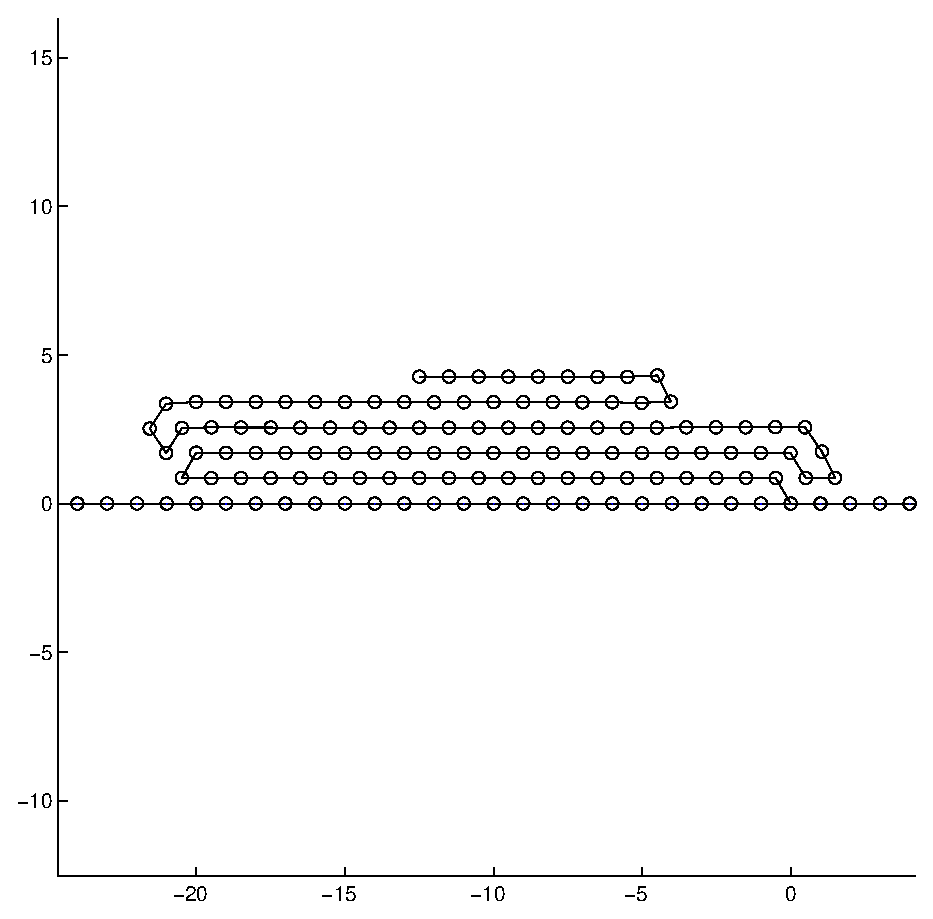
\includegraphics[scale=.4]{./fig/sims/freestanding/many_folds.eps}
			\caption{TODO \label{subfig:fs_manyfold}}
		\end{subfigure}		
		\caption{TODO\label{fig:fs_folds}}	
	\end{figure*}
	
	%% Crystalized Figures
	\begin{figure*}
		\centering
		\begin{subfigure}{.5\textwidth}
			\centering
			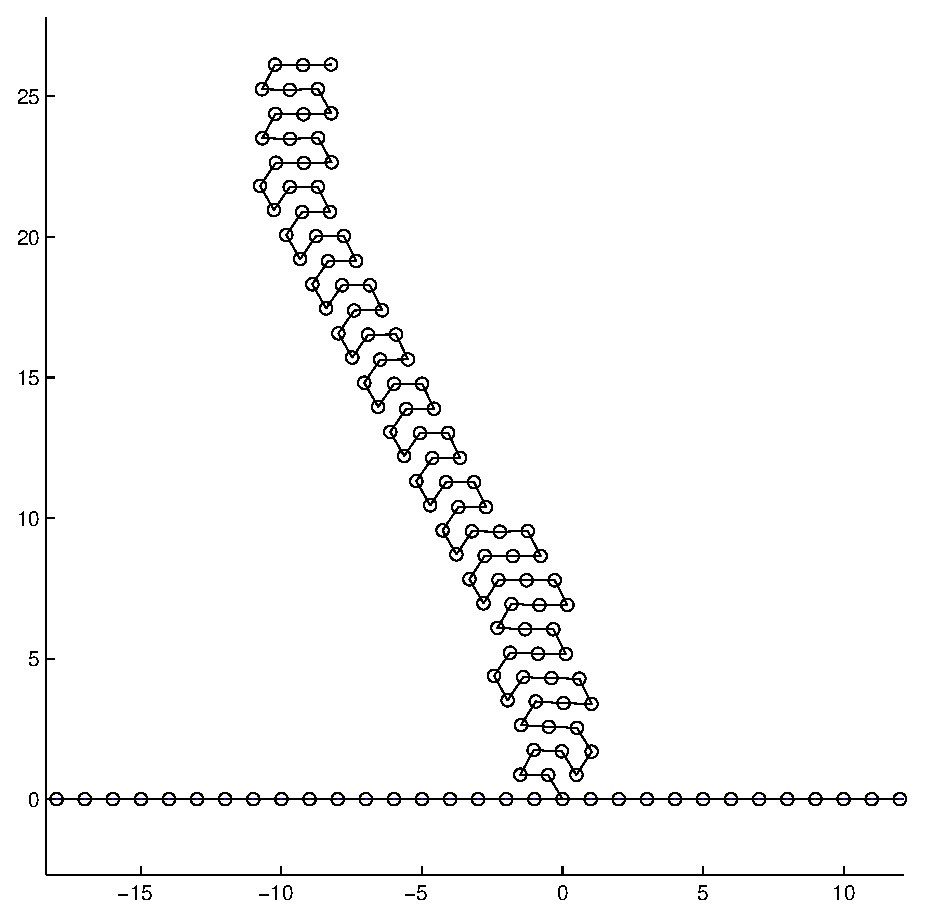
\includegraphics[scale=.4]{./fig/sims/freestanding/crystal1.eps}
			\caption{TODO \label{subfig:fs_crystal1}}
		\end{subfigure}%
		~
		\begin{subfigure}{.5\textwidth}
			\centering
			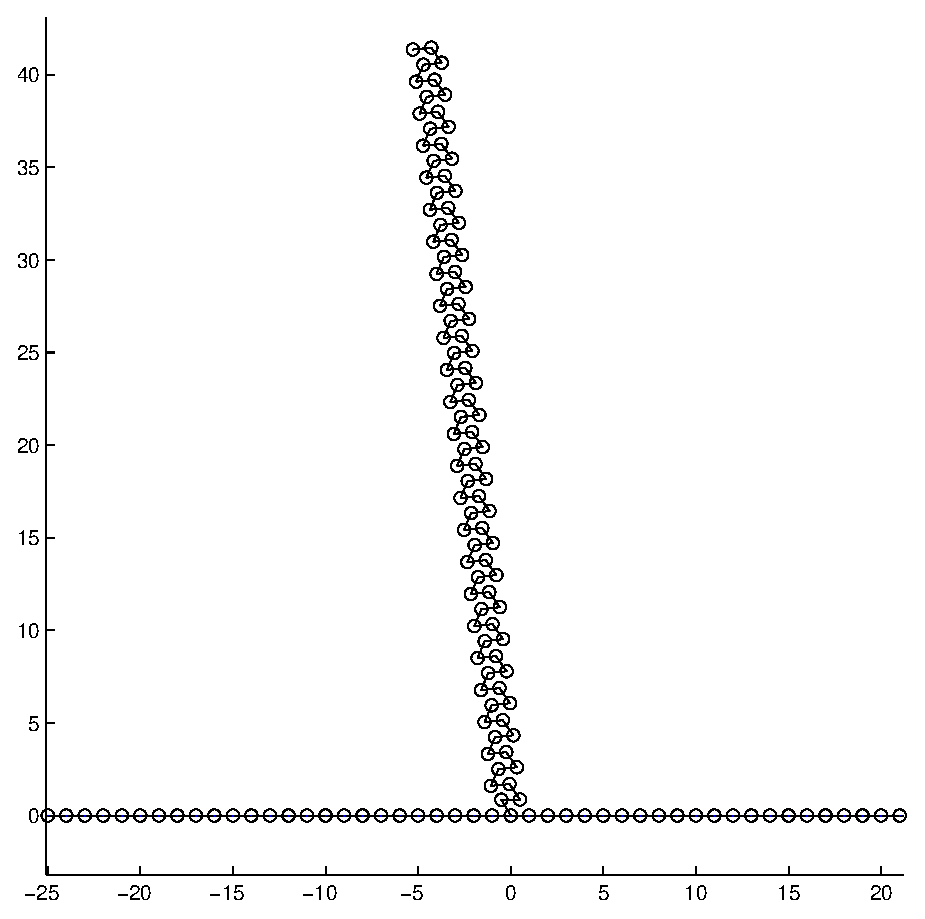
\includegraphics[scale=.4]{./fig/sims/freestanding/crystal2.eps}
			\caption{TODO \label{subfig:fs_crystal2}}
		\end{subfigure}

		\begin{subfigure}{.5\textwidth}
			\centering
			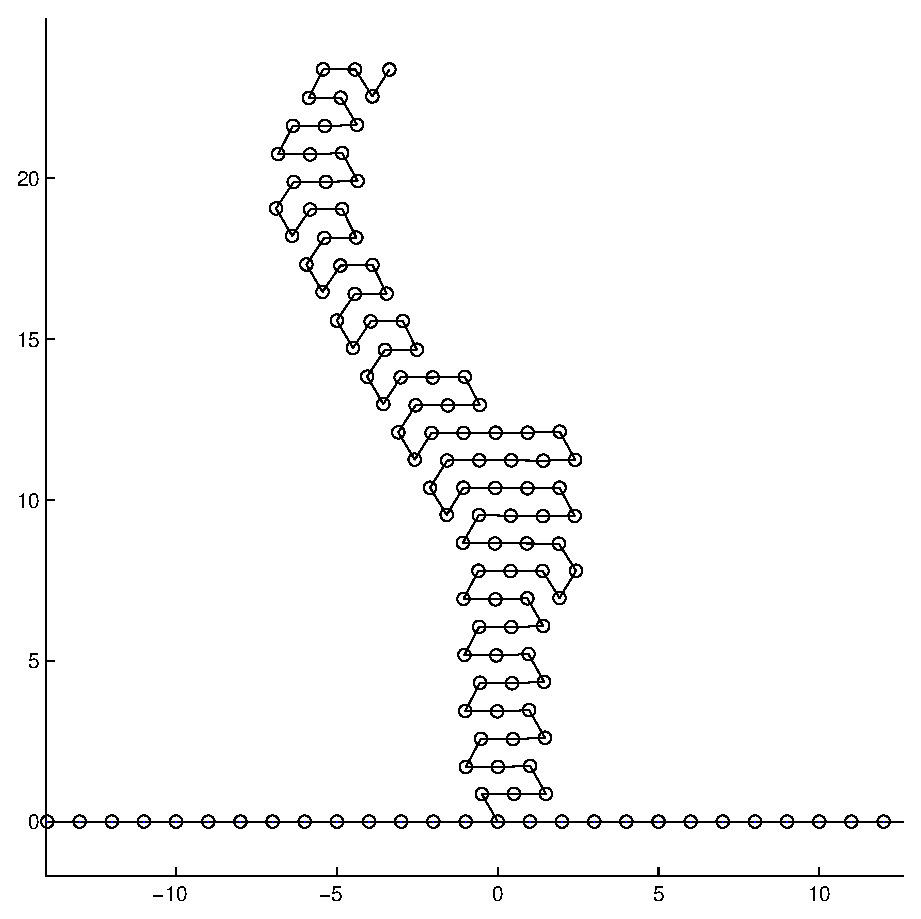
\includegraphics[scale=.4]{./fig/sims/freestanding/crystal3.eps}
			\caption{TODO \label{subfig:fs_crystal3}}
		\end{subfigure}		
		\caption{TODO\label{fig:fs_crystal}}	
	\end{figure*}

Focusing on the slanted mode it is suggested from figure \ref{fig:FreeStandingGrid} that as $\beta$ increases the ability to be slanted does so as well. If we are to look at a fiber in equilibrium near the x-axis we would see figure \ref{subfig:fs_erect} with an indistinguishable slant from being completely up right. As we increase $\eps^-$ from this position the fiber will begin to slant more dramatically. The slant in fiber will be mostly, if not completely, caused by a buckling at the root (see Fig.~\ref{subfig:fs_erectlean}). This can be understood for two reasons. First, the first particle on the fiber that can be bent by van der Waals is also closest to the bottom substrate and thus under it's greatest strain. Second, if the force pulling on the first particle is not strong enough to cause it to crystallize, then surely it will be significantly weaker for the second particle in the chain. This observation implies another important fact, namely, that if the van der Waals interaction can crystallize with the bottom substrate, then the entire fiber will collapse. The immediate change from the slanted mode to the collapsed mode is explained by this importance on the strength of the first torsional spring.
	
The continued increase in $\eps^-$ pushes the mode from slanted to collapsed and near the darkest areas we have a completely collapsed fiber (see Fig.~\ref{subfig:fs_down}). There is another sharp jump as we continue increasing $\eps^-$. The fiber switches from being completely collapsed with the bottom substrate to folding in on itself during the collapsing (see Fig.~\ref{subfig:fs_onefold}). As $\beta$ becomes too weak to maintain a stiffness to the fiber a buckle forms as it collapses. With particles on the fiber collapsing quickly the short-range nature of van der Waals leaves particles just far enough to be left "on top" of previous collapsing particles, only to quickly be taken over by the van der Waals interaction between the bottom substrate and also now the inter-fiber interaction, causing a fold. As we increase $\eps^-$ the number of folds increase as well (see Fig.~\ref{subfig:fs_manyfold}).
	
Moving towards the y-axis we find ourselves encountering a less predictable beast. With $\beta$ very weak there are several crystallization effects that happen to the fiber (see Fig.~\ref{fig:fs_crystal}). In all examples shown the crystallization is primarily inter-fiber. That is, the fiber doesn't seem to collapse, so much as crystallize with itself before it can. (TODO need precise values for these examples, and really all the above figures)

\section{Compression}

	\begin{table}
		\rowcolors{1}{}{lightgray}
		\centering
		\caption{Reference parameters for compression. \label{table:compression_reference}}
		\begin{tabular}{lcrclcr}
			$m$ & = & 1 & \hspace{1in} & $\ell_-$ & = & 1 \\
			$n$ & = & 96 & & $\ell_+$ & = & 1 \\
			$n_+$ & = & 400 & & $\ell$ & = & 1 \\
			$n_-$ & = & 200 & & $\gamma$ & = & 100 \\
			$x^{(-)}$ & = & -100 & & $\beta$ & = & 10 \\
			$y^{(-)}$ & = & 0 & & $\eps^-$ & = & 1 \\
			$x^{(+)}$ & = & -200 & & $\eps^+$ & = & 1 \\
			$y^{(+)}$ & = & 110 & & $\eps$ & = & 1 \\
			$\delta$ & = & 0 & & $\sigma$ & = & 1
		\end{tabular}
	\end{table}

	\begin{figure}[t!]
		\begin{center}
			\includegraphics[scale=1]{./fig/temp.eps}
			%\includegraphics[scale=.5]{./fig/sims/push/p.eps}
		\end{center}		
		\caption{ TODO
		\label{fig:PushGrid:vanilla}}
	\end{figure}	
	
	\begin{figure*}
		\centering
		\begin{subfigure}{.5\textwidth}
			\centering
			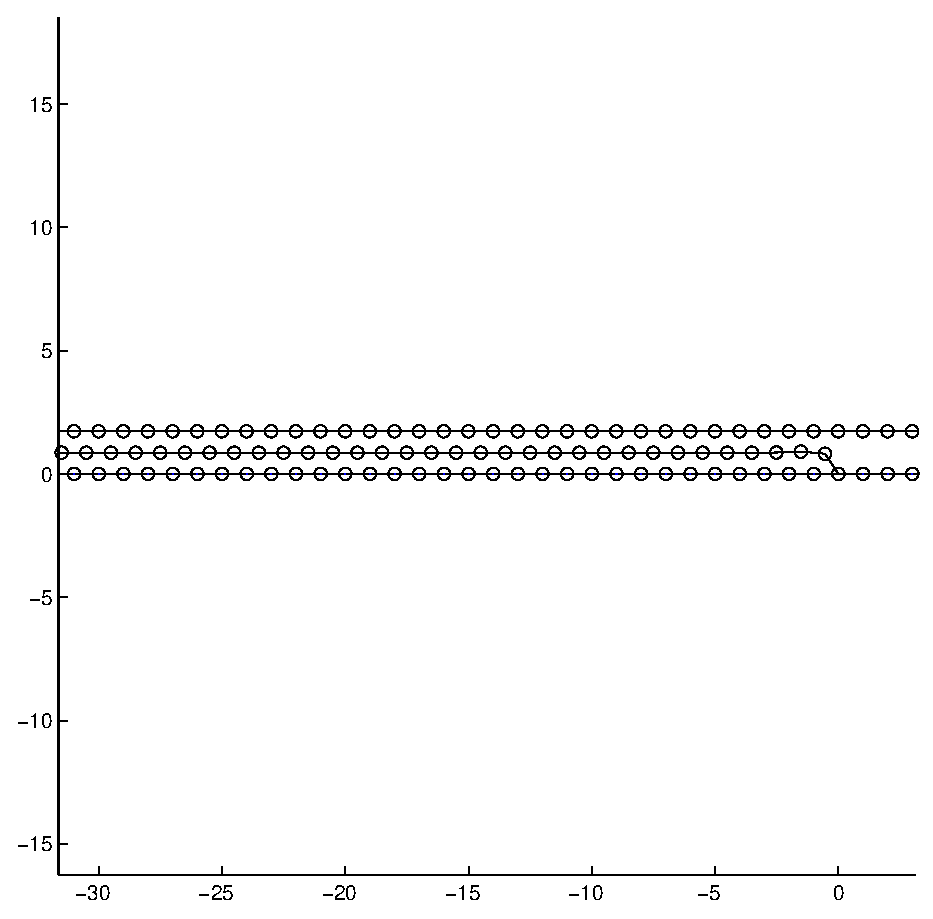
\includegraphics[scale=.4]{./fig/sims/push/squished.eps}
			\caption{TODO\label{subfig:push_squished}}
		\end{subfigure}%
		~
		\begin{subfigure}{.5\textwidth}
			\centering
			\includegraphics[scale=.4]{./fig/sims/push/one_fold.eps}
			\caption{TODO \label{subfig:push_one_fold}}
		\end{subfigure}

		\begin{subfigure}{.5\textwidth}
			\centering
			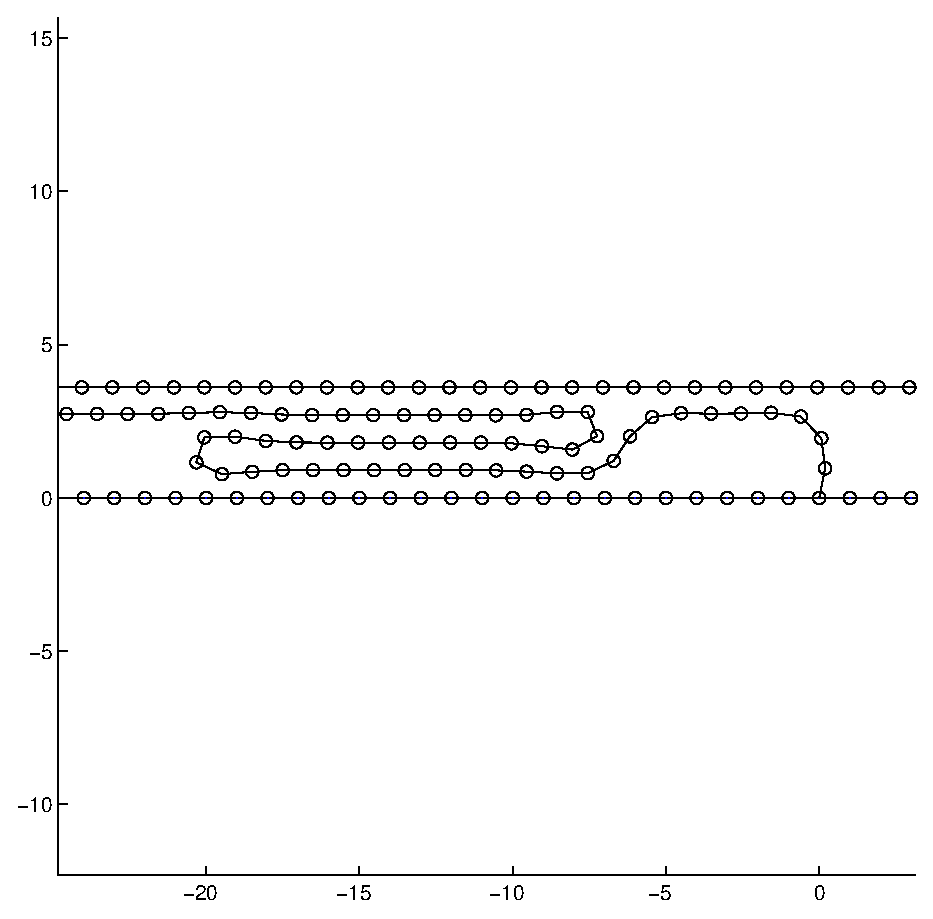
\includegraphics[scale=.4]{./fig/sims/push/two_folds.eps}
			\caption{TODO\label{subfig:push_two_folds}}
		\end{subfigure}
		\caption{TODO\label{fig:push_fold}}
	\end{figure*}

	\begin{figure*}
		\centering
		\begin{subfigure}{.5\textwidth}
			\centering
			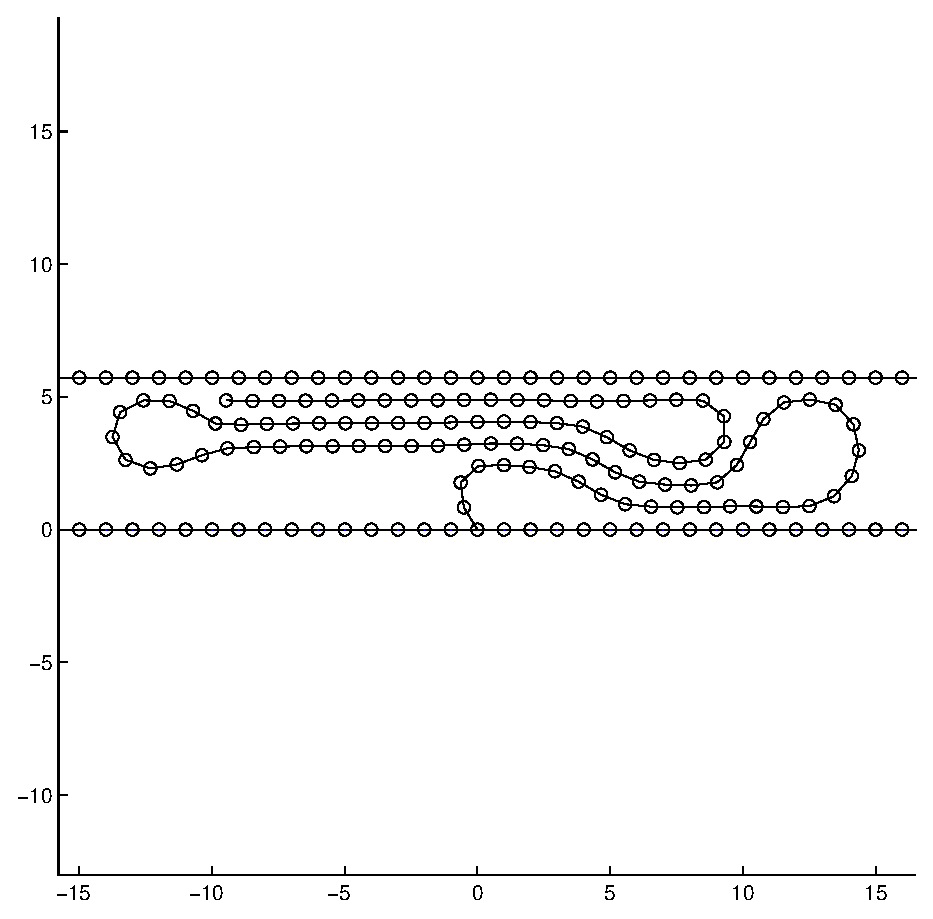
\includegraphics[scale=.4]{./fig/sims/push/curled1.eps}
			\caption{TODO \label{subfig:push_curled1}}
		\end{subfigure}%
		~
		\begin{subfigure}{.5\textwidth}
			\centering
			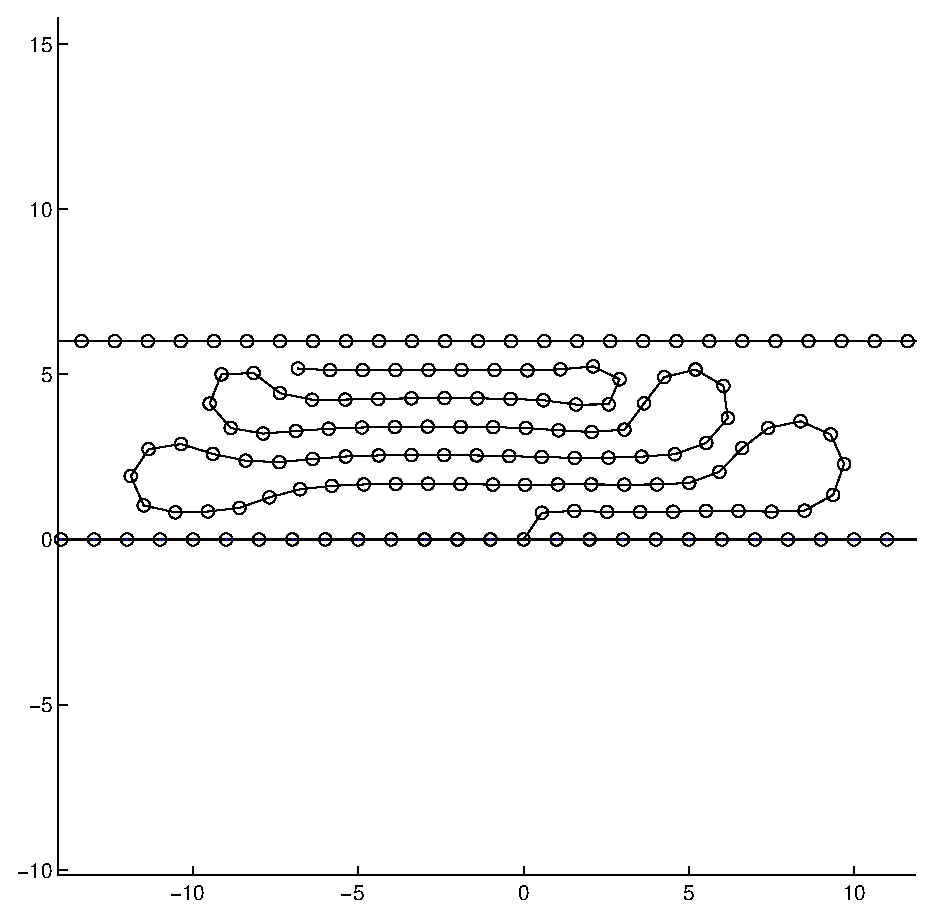
\includegraphics[scale=.4]{./fig/sims/push/curled2.eps}
			\caption{TODO\label{subfig:push_curled2}}
		\end{subfigure}
		\caption{TODO\label{fig:push_curled}}
	\end{figure*}

The compression of a fiber by a load is likely to cause it to buckle. We investigate here under what parameters it will buckle and how it buckles. In all simulations the fiber starts standing vertically and in equilibrium (under the equilibrium criteria described in Chapter~\ref{chap:two}). The top substrate starts a distance far enough away from the fiber so that the cut off Lennard-Jones prevents it from interacting. The experiment begins with a load on the top substrate moving it towards the fiber and bottom substrate. In every configuration we have found under this experiment there is some degree of crystallization between particles on the fiber and particles on the top substrate. Therefore we use the adhesion metric (see Equation~\ref{eqn:adhesion:top}) to differentiate between different buckling configurations. All experiments are done against a set of reference parameters (see Table~\ref{table:compression_reference}). These values have minor significance; a value is chosen to be one unless there is otherwise reason not to. The starting position and particle count for substrates are chosen so that if a fiber were to collapse under any extreme it doesn't run out of particles on either substrate to interact with. This is a guarantee for the bottom substrate based on the chosen values but the top substrate can still ``miss'' the fiber since it has only finitely many particles. Both $\gamma$ and $\beta$ were selected to keep the fiber vertical when not under load, and $\delta$ was chosen to be zero for aesthetics.

\subsection{Observations of Reference Parameters}

Given the reference parameters in Table~\ref{table:compression_reference} we have a diagram, Figure~\ref{fig:PushGrid:vanilla}, demonstrating different buckling configurations after the system is in equilibrium. There is one configuration we focus on in detachment specifically that we can observe. The fiber is said to be \textit{flattened} between the top and bottom substrate when it has completely crystallized with the top substrate and no torsional spring, with the exception of the root, is bent (see Figure~\ref{subfig:push_squished}). This is the starting configuration, after relaxation, for the detachment experiment. Figure~\ref{fig:PushGrid:vanilla} also demonstrates a relationship between an angled load and a flattened configuration. The fiber is said to have a \textit{fold} when one or more particle of the fiber has crystallized with other particles on the fiber. When the load is near $\frac{\pi}{2}$ we start to see folds (see Figure~\ref{fig:push_fold}). When the substrate is even closer, or directly down, the fiber starts to buckle immediately causing more folds in configurations as shown in Figure~\ref{fig:push_curled}.

Flattened fibers occur under these parameters when the angle of the load is sufficiently away from $\frac{\pi}{2}$. An explanation for this behavior is that as the fiber buckles it crystallizes with the top substrate and is sheared by the horizontal component of the load to be ``zipped'' to the top substrate. A fiber \textit{zips} (or \textit{unzips}) from a substrate when one particle crystallizes (or breaks crystallization) at a time and in rapid succession. Therefore if the load is closer to $\frac{\pi}{2}$ it loses the shearing component and no longer causes the fiber to zip.

	\begin{figure}
		\begin{center}
			\includegraphics[scale=.5]{./fig/sims/push_b100/p.eps}
		\end{center}		
		\caption{ TODO
		\label{fig:PushGrid:b100}}
	\end{figure}	
	
	\begin{figure}
		\begin{center}
			\includegraphics[scale=.5]{./fig/sims/push_b1000/p.eps}
		\end{center}		
		\caption{ TODO
		\label{fig:PushGrid:b1000}}
	\end{figure}
	
	\begin{figure*}
		\centering
		\begin{subfigure}{.5\textwidth}
			\centering
			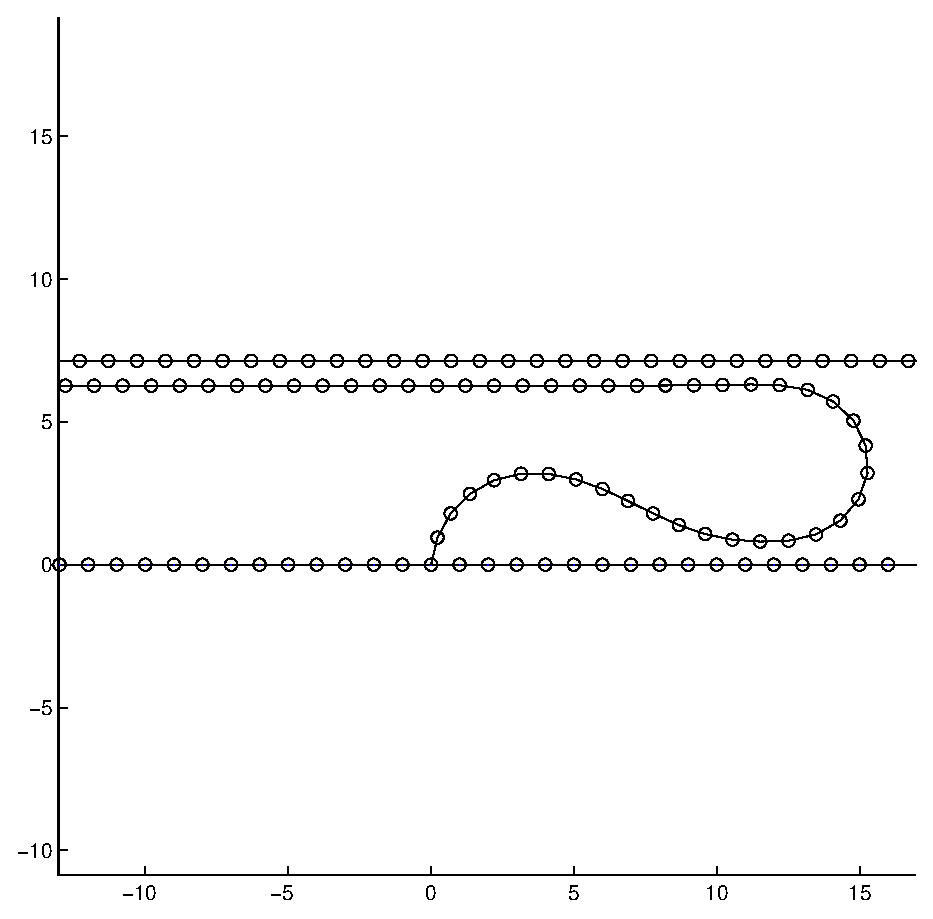
\includegraphics[scale=.4]{./fig/sims/push_b100/low_mag.eps}
			\caption{TODO \label{subfig:push_b100_low_mag}}
		\end{subfigure}%
		~
		\begin{subfigure}{.5\textwidth}
			\centering
			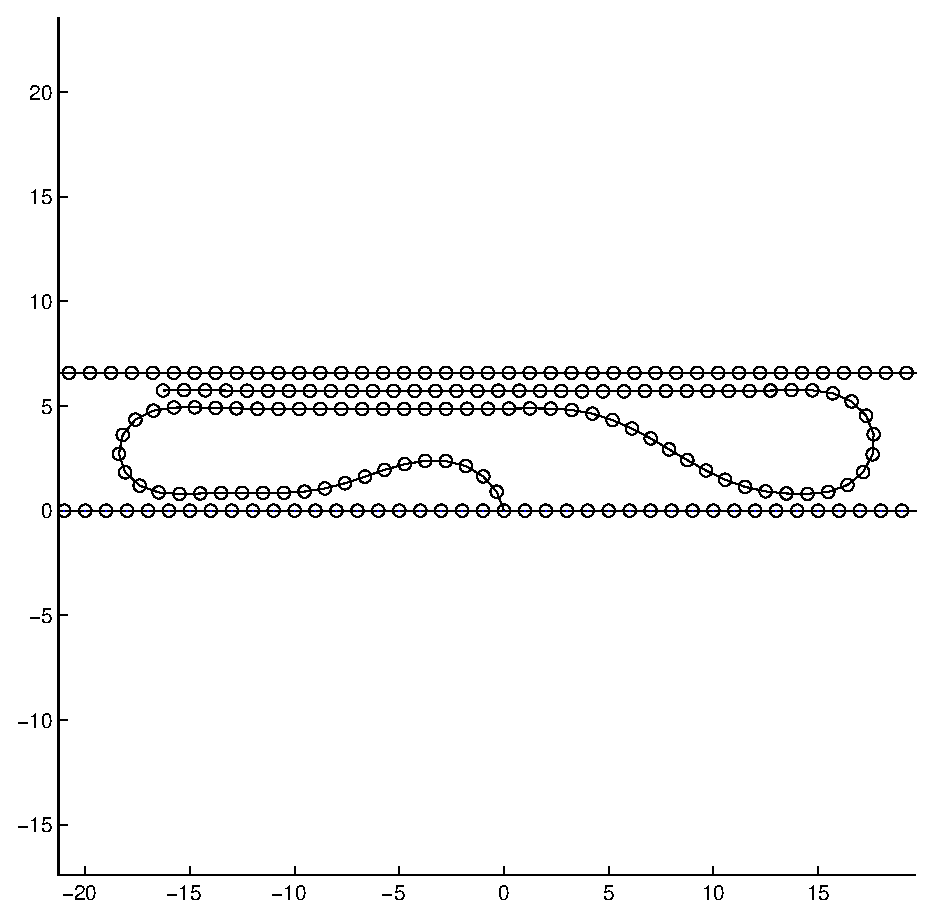
\includegraphics[scale=.4]{./fig/sims/push_b100/high_mag.eps}
			\caption{TODO \label{subfig:push_b100_high_mag}}
		\end{subfigure}

		\begin{subfigure}{.5\textwidth}
			\centering
			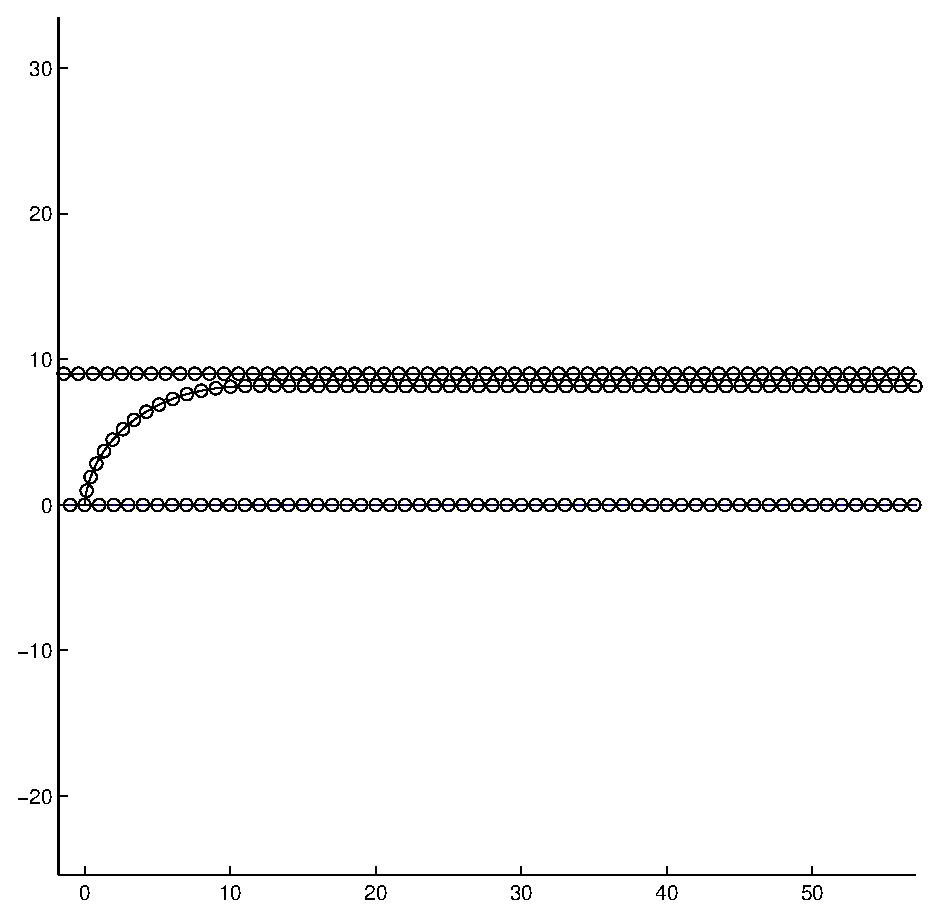
\includegraphics[scale=.4]{./fig/sims/push_b1000/bend.eps}
			\caption{TODO \label{subfig:push_b1000_bend}}
		\end{subfigure}		
		\caption{TODO\label{fig:push_bending}}	
	\end{figure*}

\subsection{Observations Increasing $\beta$}

Increasing $\beta$ shows a shrinking region for folding fibers under any load in Figure~\ref{fig:PushGrid:b100} and Figure~\ref{fig:PushGrid:b1000}. This suggests that folding in a fiber is a relation between $\beta$ and van der Waals (i.e. $\eps$ and $\eps^+$). The explanation being that folds can only occur when the top substrate is not causing the fiber to zip, either by load or overpowering van der Waals, and when $\beta$ is weak enough. If $\beta$ is strong enough to prevent folding it would suggest that the torsional springs are breaking crystallization with the top substrate as it compresses the fiber to shift more particles against the top substrate. As $\beta$ increases it would then become strong enough to break increasingly more crystallized particles with the top substrate to prevent a fold. Figure~\ref{subfig:push_b100_low_mag} and Figure~\ref{subfig:push_b100_high_mag} show configurations of different magnitude at $\beta = 10$ and how folds can still occur. Figure~\ref{subfig:push_b1000_bend} shows a configuration where no folding occurs. We also see that sufficiently strong $\beta$ and sufficiently weak magnitude of the load prevent a flattened configuration. We would expect the number of particles on the fiber that adhere to the top substrate to reduce if we continued to increase $\beta$. 

	\begin{figure}
		\begin{center}
			\includegraphics[scale=.5]{./fig/sims/push_eb0.1/p.eps}
		\end{center}		
		\caption{ TODO
		\label{fig:PushGrid:eb0.1}}
	\end{figure}	

	\begin{figure}
		\begin{center}
			\includegraphics[scale=.5]{./fig/sims/push_et0.1/p.eps}
		\end{center}		
		\caption{ TODO
		\label{fig:PushGrid:et0.1}}
	\end{figure}
	
	\begin{figure}
		\begin{center}
			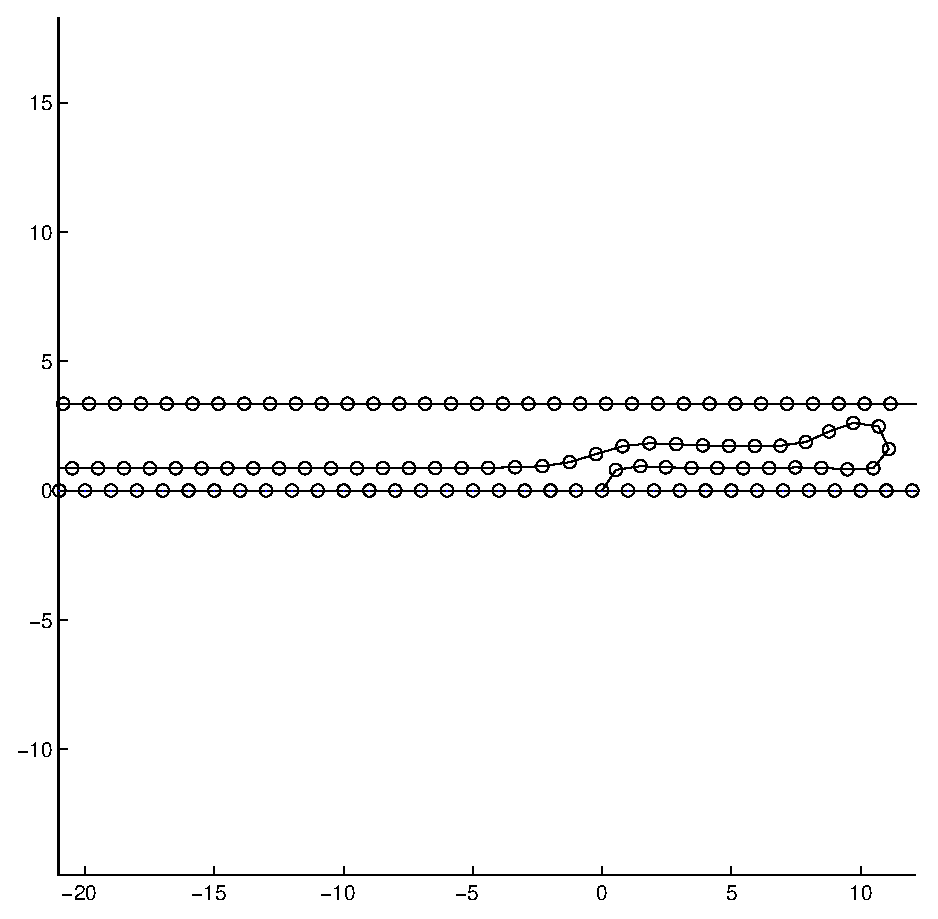
\includegraphics[scale=.4]{./fig/sims/push_et0.1/hump.eps}
		\end{center}		
		\caption{ TODO
		\label{fig:push_hump}}
	\end{figure}	

	\begin{figure}
		\begin{center}
			\includegraphics[scale=.5]{./fig/sims/push_eb0.1_et0.1/p.eps}
		\end{center}		
		\caption{ TODO
		\label{fig:PushGrid:eb0.1_et0.1}}
	\end{figure}	

	\begin{figure*}
		\centering
		\begin{subfigure}{.5\textwidth}
			\centering
			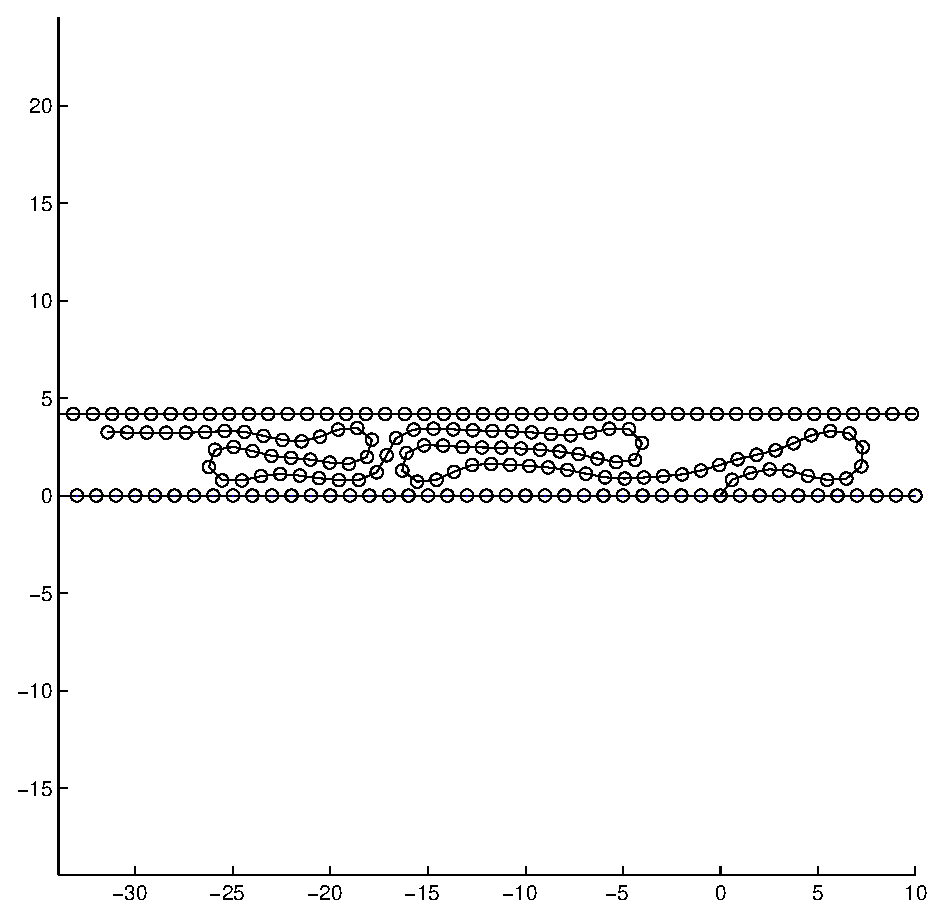
\includegraphics[scale=.4]{./fig/sims/push_eb0.1_et0.1/crumple.eps}
			\caption{TODO \label{subfig:push_crumple}}
		\end{subfigure}%
		~
		\begin{subfigure}{.5\textwidth}
			\centering
			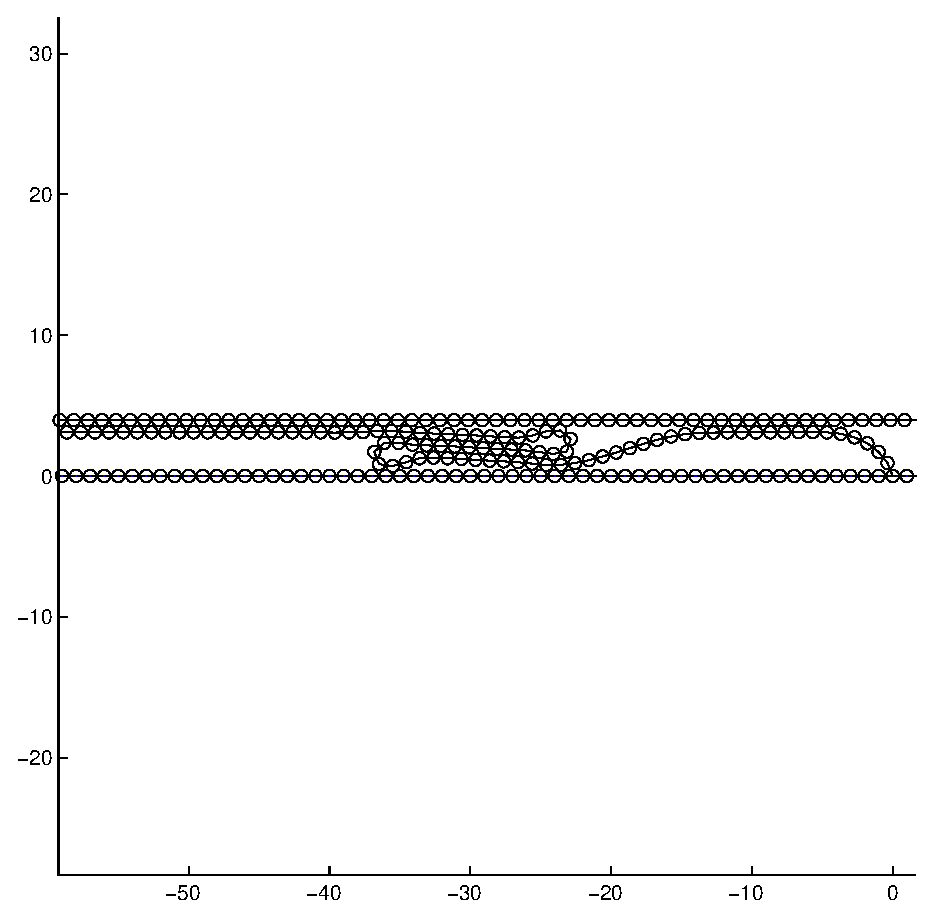
\includegraphics[scale=.4]{./fig/sims/push_eb0.1_et0.1/crumple2.eps}
			\caption{TODO \label{subfig:push_crumple2}}
		\end{subfigure}

		\begin{subfigure}{.5\textwidth}
			\centering
			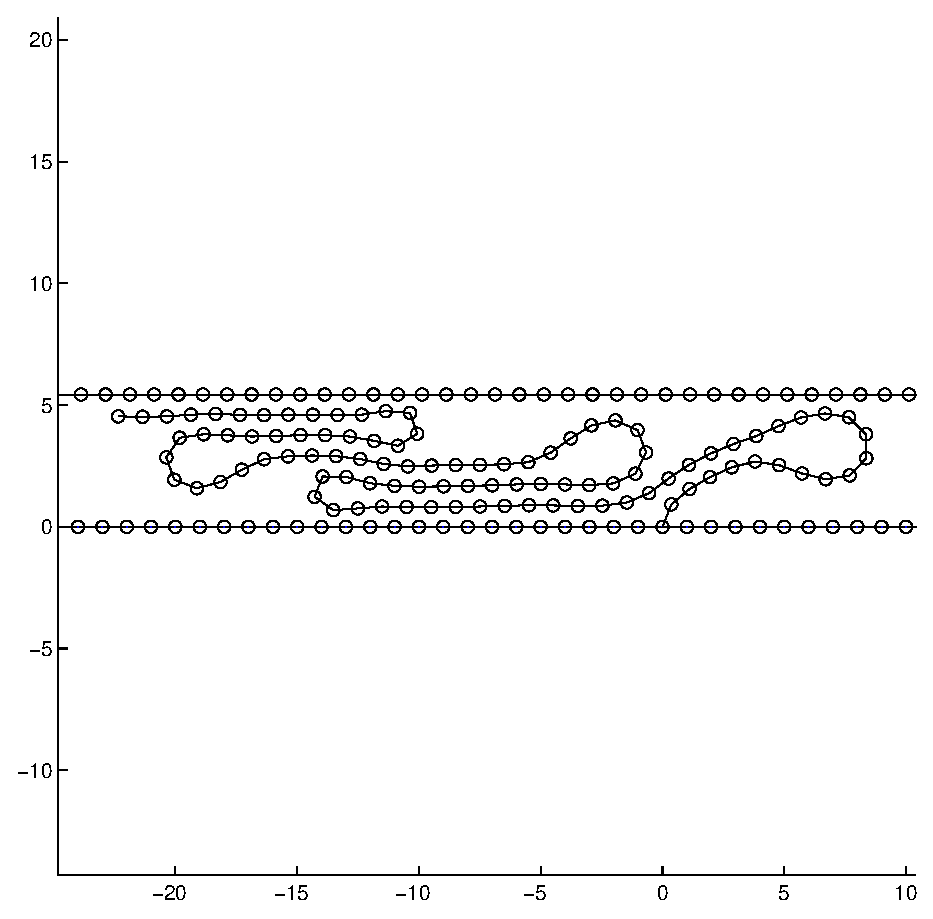
\includegraphics[scale=.4]{./fig/sims/push_eb0.1_et0.1/crumple3.eps}
			\caption{TODO \label{subfig:push_crumple3}}
		\end{subfigure}		
		\caption{TODO\label{fig:push_crumple}}	
	\end{figure*}

\subsection{Observations Decreasing $\eps^-$ and $\eps^+$} \label{subsection:push:eps}

An order of magnitude decrease in $\eps^-$ seems to play no qualitative role in equilibrium configurations, at least with the selected reference parameters (see Figure~\ref{fig:PushGrid:eb0.1}). However, an order of magnitude decrease in $\eps^+$ plays a significant role (see Figure~\ref{fig:PushGrid:et0.1}). The shear component of the load instead of causing the fiber to zip to the top substrate causes the top substrate to slide off. That is, the van der Waals interaction is not strong enough for large shear components or large magnitudes to hold or adhere to the fiber. Even so and angled load is necessary to cause a flattened configuration, but the region of angles that cause folding as increased. This is because with sufficiently small shear component will cause the fiber to buckle and then van der Waals interaction between particles on the fiber will be the dominate force as the fiber zips against itself. The isolated white regions of Figure~\ref{fig:PushGrid:et0.1} are of a ``hump'' configuration (see Figure~\ref{fig:push_hump}). The hump is caused by the fiber zipping to the bottom substrate with fold immediately at the root causing a ``hump''. The top substrate is then only adhered to a single particle of the fiber. If both $\eps^-$ and $\eps^+$ are decreased by an order of magnitude then we have a similar diagram as with only $\eps^-$ being reduced but the ``hump'' configuration is lost (see Figure~\ref{fig:PushGrid:eb0.1_et0.1}). This variation from the reference parameters weakens adhesion of all van der Waals interactions between the fiber and either substrate but keeps the same interaction between particles on the fiber with other particles on the fiber. Therefore, folding is more prominent for the same reasons that folding was more prominent when only $\eps^-$ was decreased.
	
	\begin{figure}
		\begin{center}
			\includegraphics[scale=.5]{./fig/sims/push_g1000/p.eps}
		\end{center}		
		\caption{ TODO
		\label{fig:PushGrid:g1000}}
	\end{figure}	

\subsection{Observations Increasing $\gamma$}

An order of magnitude increase in $\gamma$ has no observable effect (see Figure~\ref{fig:PushGrid:g1000}). The purpose of $\gamma$ is to keep the particles a fixed distance apart but allow for some relaxation. If $\gamma$ were very large we might expect the bonds to be too stiff and prevent crystallization. However, the uniform spacing between particles on the substrates and the ideal spacing, $\ell$, of particles on the fiber allow for at least some crystallization regardless of how stiff the extensible spring is made to be. Intuitively, it would seem that even with very stiff extensible springs the diagram would still not vary significantly from Figure~\ref{fig:PullGrid}.

	\begin{figure}
		\begin{center}
			\includegraphics[scale=.5]{./fig/sims/push_p1_oscount0/p.eps}
		\end{center}		
		\caption{ TODO
		\label{fig:PushGrid:p1}}
	\end{figure}

\subsection{Replacing Atomized Bottom Substrate with Pressure}

Up until now all experiments have been done with a bottom substrate comprised of contiguous particles. However, varying the van der Waals strength of these particles with particles of the fiber didn't have any qualitative effect as shown in Subsection~\ref{subsection:push:eps}. We might ask if particles on the bottom substrate are necessary at all to the behavior of the fiber. Thus, we remove all particles on the bottom substrate and replace the van der Waals interaction with a pressure (see Figure~\ref{fig:PushGrid:p1}. \textbf{TODO}(introduce the equation here? In Chapter 2?) We can see some general similarities between the reference diagram and a bottom substrate replaced with pressure. However, there are also some noticeable anomalies. There are ``hump'' like configurations and different folding behavior. \textbf{TODO}(I don't have an explanation)

%How the fiber deforms under compression, in particular the amount of the fiber under contact, is a question that has been asked and answered in other contexts
\textbf{TODO}(Cite Majidi and He).

\section{Detachment}

	\begin{table}
		\rowcolors{1}{}{lightgray}
		\centering
		\caption{Reference parameters for compression. \label{table:detachment_reference}}
		\begin{tabular}{lcrclcr}
			$m$ & = & 1 & \hspace{1in} & $\ell_-$ & = & 1 \\
			$n$ & = & 96 & & $\ell_+$ & = & 1 \\
			$n_+$ & = & 300 & & $\ell$ & = & 1 \\
			$n_-$ & = & 300 & & $\gamma$ & = & 100 \\
			$x^{(-)}$ & = & -150 & & $\beta$ & = & 1 \\
			$y^{(-)}$ & = & 0 & & $\eps^-$ & = & 1 \\
			$x^{(+)}$ & = & -150 & & $\eps^+$ & = & 1 \\
			$y^{(+)}$ & $\approx$ & 1.72741 & & $\eps$ & = & 1 \\
			$\delta$ & = & 0 & & $\sigma$ & = & 1
		\end{tabular}
	\end{table}
	
	\begin{figure}[h]
		\begin{center}
			\includegraphics[scale=.5]{./fig/sims/pull/p.eps}
		\end{center}		
		\caption{ TODO
		\label{fig:PullGrid}}
	\end{figure}
	
	\begin{figure}[h]
		\begin{center}
			\includegraphics[scale=.5]{./fig/sims/pull_b10/p.eps}
		\end{center}		
		\caption{ TODO
		\label{fig:PullGrid:b10}}
	\end{figure}
	
	\begin{figure}[h]
		\begin{center}
			\includegraphics[scale=.5]{./fig/sims/pull_b100/p.eps}
		\end{center}		
		\caption{ TODO
		\label{fig:PullGrid:b100}}
	\end{figure}
	
	\begin{figure}[h]
		\begin{center}
			\includegraphics[scale=.5]{./fig/sims/pull_eb0.1/p.eps}
		\end{center}		
		\caption{ TODO
		\label{fig:PullGrid:eb0.1}}
	\end{figure}

	\begin{figure}[h]
		\begin{center}
			\includegraphics[scale=.5]{./fig/sims/pull_eb0.01/p.eps}
		\end{center}		
		\caption{ TODO
		\label{fig:PullGrid:eb0.01}}
	\end{figure}
	
	\begin{figure}[h]
		\begin{center}
			\includegraphics[scale=.5]{./fig/sims/pull_eb0/p.eps}
		\end{center}		
		\caption{ TODO
		\label{fig:PullGrid:eb0}}
	\end{figure}
	
	\begin{figure}[h]
		\begin{center}
			\includegraphics[scale=.5]{./fig/sims/pull_eb0.1_et0.1/p.eps}
		\end{center}		
		\caption{ TODO
		\label{fig:PullGrid:eb0.1_et0.1}}
	\end{figure}
	
	\begin{figure}[h]
		\begin{center}
			\includegraphics[scale=.5]{./fig/sims/pull_eb0.1_et0.1_e0.1/p.eps}
		\end{center}		
		\caption{ TODO
		\label{fig:PullGrid:eb0.1_et0.1_e0.1}}
	\end{figure}
	
	\begin{figure}[h]
		\begin{center}
			\includegraphics[scale=.5]{./fig/sims/pull_et10/p.eps}
		\end{center}		
		\caption{ TODO
		\label{fig:PullGrid:et10}}
	\end{figure}
	
	\begin{figure}[h]
		\begin{center}
			\includegraphics[scale=.5]{./fig/sims/pull_g1000/p.eps}
		\end{center}		
		\caption{ TODO
		\label{fig:PullGrid:g1000}}
	\end{figure}
	
	\begin{figure}[h]
		\begin{center}
			\includegraphics[scale=.5]{./fig/sims/pull_p1_oscount0/p.eps}
		\end{center}		
		\caption{ TODO
		\label{fig:PullGrid:p1}}
	\end{figure}
	
	\begin{figure}[h]
		\begin{center}
			\includegraphics[scale=.5]{./fig/sims/pull_p10_oscount0/p.eps}
		\end{center}		
		\caption{ TODO
		\label{fig:PullGrid:p10}}
	\end{figure}


\subsection{Observations of Reference Parameters}

\subsection{Observations Increasing $\beta$}

\subsection{Observations Decreasing $\eps^-$}

\subsection{Observations Decreasing $\eps^-$, $\eps^+$, and $\eps$}

\subsection{Observations Increasing $\eps^+$}

\subsection{Observations Increasing $\gamma$}

\subsection{Replacing Atomized Bottom Substrate with Pressure}




\section{Conclusions}